\documentclass[conference]{IEEEtran}
\IEEEoverridecommandlockouts
% The preceding line is only needed to identify funding in the first footnote. If that is unneeded, please comment it out.
\usepackage{cite}
\usepackage{amsmath,amssymb,amsfonts}
\usepackage{algorithmic}
\usepackage{graphicx}
\usepackage{textcomp}
\usepackage{xcolor}
\def\BibTeX{{\rm B\kern-.05em{\sc i\kern-.025em b}\kern-.08em
    T\kern-.1667em\lower.7ex\hbox{E}\kern-.125emX}}
\begin{document}

\title{Readability Score Classification of Computer Science Publications using Neural Network\\
}

\author{\IEEEauthorblockN{Alfredo J. Peña}
\IEEEauthorblockA{\textit{Department of Computer Science} \\
\textit{University of Texas Rio Grande Valley}\\
Edinburg, Texas \\
alfredo.pena01@utrgv.edu}
\and
\IEEEauthorblockN{Amit Das}
\IEEEauthorblockA{\textit{Department of Computer Science} \\
\textit{University of Texas Rio Grande Valley}\\
Edinburg, Texas \\
amit.das01@utrgv.edu}
\and
\IEEEauthorblockN{Md Shahriar Forhad}
\IEEEauthorblockA{\textit{Industrial \& Manufacturing Engineering} \\
\textit{University of Texas Rio Grande Valley}\\
Edinburg, Texas \\
mdshahriar.forhad01@utrgv.edu}
}

\maketitle

\begin{abstract}
Readability is an important aspect for scientific publications since it helps transmit knowledge and ensures that results are reproducible. Machine-assisted text analysis has been around for a long time. We aim to take it a step further by employing deep learning based neural networks to quantify readability in computer science publications. We used a corpus of 322,563 abstracts published between 1913 and 2020 from the Scopus database, and proposed a deep learning model that analyzes the readability of abstracts and delivers a score. 
\end{abstract}

\begin{IEEEkeywords}
readability, neural, network, score, publications
\end{IEEEkeywords}

\section{Introduction}
Artificial Intelligence (AI) and Machine Learning (ML) have provided new dimensions in many fields due to their unparalleled processing capabilities. We'll employ that processing power to investigate the readability of publications in this case.
\par
The ability to comprehend the text material readily and rapidly is defined as text readability \cite{b1}. The purpose of readability analysis is to assign a score to a paper's difficulty for average readers. Most ways for autonomously measuring the difficulty of articles are based on two aspects: the difficulty of syntax and the complexity of the lexical items \cite{b2}. Previous works \cite{b3} \cite{b4} depend on explicit metrics like Average Syllables Per Word, Mean Words Per Sentence, and so on to define these aspects. The Flesch-Kincaid score is a quantitative metric that is defined as a linear combination of these components \cite{b5}. Later methods mostly focus on proposing additional features, with the most recent CohMetrix 3.0 \cite{b6} proposing 108, and they aggregate and utilize the features by using linear functions or statistical approaches such as Support Vector Machine (SVM) or multilayer perceptron \cite{b7}\cite{b8}\cite{b9}\cite{b10}\cite{b11}. While these approaches offer some advantages, as well as a number of disadvantages too. Particularly, these methods do not incorporate sequential and structural information, and they do not capture implicit yet critical semantics at the word or sentences level \cite{b2}.
\par
There have been lots of studies on using neural models for sentimental or subject document classification or ranking, but very few have focused on the readability analysis. Despite topic and sentiment-related document classification tasks, which focus on utilizing sections of lexical items that are important to the document's overall meanings and sentiment, readability analysis necessitates the aggregate of difficulty across all sentence components. Additionally, accurately capturing text readability necessitates the model's incorporation of extensive readability-aware elements, such as complexity, sequence, and structural information, into the appropriate learning model. As a result, several methodologies must be investigated in order to gain a better knowledge of text difficulty and the various aspects that influence it.
\par
We look into an alternate approach on how to estimate document difficulty based on the structure of words and sentences in this work. We address key earlier work in the parts that follow, outline our data collection process, and present our study's findings.

\section{Problem Statement}
A paper from the Karolinska Institutet in Sweden suggests that the readability of scientific texts is trending down overall and being filled with more and more jargon every year\cite{b12}.

\begin{figure}[htbp]
\centerline{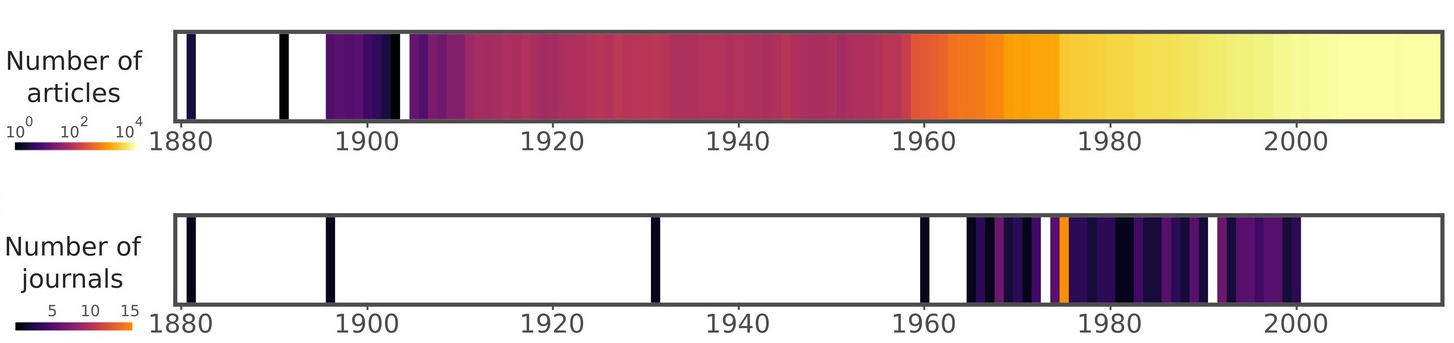
\includegraphics[width=200pt]{images/articles_up.png}}
\caption{Articles and Journals from 1880 to 2017\cite{b12}.}
\label{articles_up}
\end{figure}

\begin{figure}[htbp]
\centerline{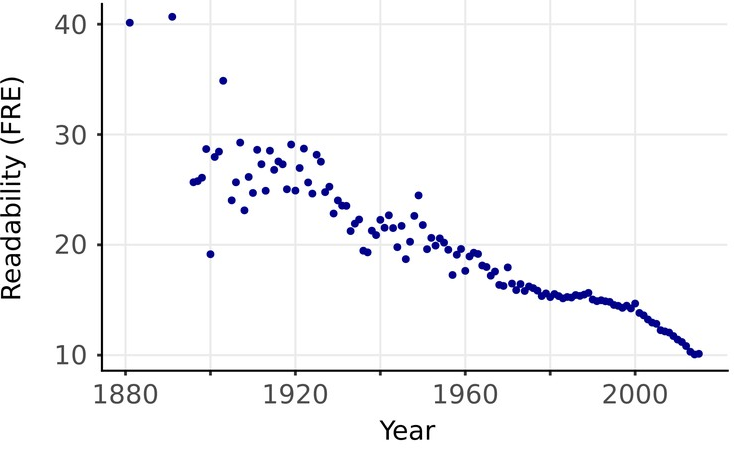
\includegraphics[width=200pt]{images/read_down.png}}
\caption{Mean Flesch Reading Ease (FRE) readability for each year\cite{b12}.}
\label{readability_down}
\end{figure}

\par
This type of trend may jeopardize the availability of research papers to the general public and even to inter field research. The less we can understand one another the less progress we make. Although the advancement of technology over the years may suggest that there is no need to fix this readability problem, we can also assume we have simply not hit the point where we can no longer understand ourselves with ease.
\par
Readability being such an important attribute for a well-written paper in any field makes study with Deep Learning practices more enticing. Passing a paper through machine eyes to quantify readability will prove a useful asset for future development.

\section{Data and Methods}
We built a new dataset from Scopus, the world's largest collection of scholarly papers, for this study. From the database, we have hand curated articles of various subfields in the fields of computer science up until this point. This data took a significant amount of time to generate.

\subsection{Data Collection Procedure} \label{datashake}
We have downloaded about 1.7 million Computer science publications data from Scopus.  It takes around three weeks to complete the downloading process. We have to collect these data with maximum of 2000 abstract at a time. It was a very tedious process. Data collection process was a cycle:
\begin{center}
Download $\rightarrow$ Upload $\rightarrow$ Merge $\rightarrow$ Repeat
\end{center}
\par
After that we have Selected only AI/ML Papers for these projects. We have selected these publications by Matching the Hand curated keywords. The Keywords are:
\par
\begin{footnotesize}
\textit{Artificial Intelligence, Experts System, Automatic Speech Recognition, Caffe Deep Learning Framework, Chatbot, Computational Linguistics, Computer Vision, Data Mining, Decision Trees, Deep Learning, Deeplearning4j, Distinguo, Deep Representation Learning, Google Cloud Machine Learning, convolutional neural networks, Pattern Recognition, Support Vector Machine, Robotics, Knowledge Discovery and Data Mining, Advances in Neural Information Processing Systems, Gradient boosting, H2O (software), IBM Watson, Image Processing, Image Recognition, ImageNet, Resnet, Keras, Knowledge based systems, Latent Dirichlet Allocation, Latent Semantic Analysis, Lexalytics, Lexical Acquisition, Lexical Semantics, Libsvm, LSTM, Machine Learning, Machine Translation, Machine Vision, Madlib, Mahout, Microsoft Cognitive Toolkit, MLPACK, Mlpy, Modular Audio Recognition Framework, Moses, MXNet, Natural Language Processing, Natural Language Toolkit (NLTK), natural language understanding, ND4J (software), Natural Language Learning, Nearest Neighbor Algorithm, data clustering, Neural Networks, Object Recognition, Object Tracking, OpenCV, OpenNLP, Pattern Recognition, Pybrain, Random Forests, Recommender Systems, Language Model, Semantic Driven Subtractive Clustering Method, Semi-Supervised Learning, Sentiment Analysis, Opinion Mining, Sentiment Classification, Speech Recognition, Supervised Learning, Support Vector Machines, TensorFlow, Text Mining, Text to Speech, Tokenization, topic model, Unsupervised Learning, Virtual Agents, Vowpal, Wabbit, Word2Vec, Word Embedding, Xgboost, AI ChatBot, conversational agent, Robotic, Learning Representations, Boltzmann Machine, AI KIBIT, ANTLR, Apertium, Hidden Markov Model, sequence model, Supervised Learning, generative adversarial network, Reinforcement Learning,Attention Mechanism, Auto Encoder, Auto Regressive Model, Autoencoder, BERT, Back Propagation, Backpropagation, Bidirectional Encoder Representations, Boltzmann Machine, Chainer, Convolutional Network, Deep Architecture, Deep Autoencoder, Deep Belief Network, Deep Convolutional, Deep Deterministic Policy Gradient, Deep Embedding, Deep Encoder Decoder, Deep Generative Model, Deep Generative Network, Deep Hashing Method, Deep Learning, Deep Linear Network, Deep Metric Learning, Deep Model, Deep Network, Deep Probabilistic Model, Deep Q Learning, Deep Q Network, Deep Recurrent Network, Deep Reinforcement Learning, Deep Representation Learning, Deep Supervised Hashing, Deeplearning4j, Depth Wise Convolution, DyNet, Encoder Decoder,  Gated Recurrent Unit, Generative Adversarial Net, Generative Adversarial Network, GloVe, Gluon, Gradient Descent, Graphics Processing Unit, GraspNET, Hopfield Network, Keras, LSTM, Lasagne, Liquid State Machine, Long Short Term Memory, Max Pooling, Microsoft Cognitive Toolkit, Multilayer Perceptron, Mxnet, Neural Architecture, Neural Language Model, Neural Machine Translation, Neural Model, Neural Net, Neural Network, Neural Style Transfer, Neural Turing Machine, ONNX, OpenNN, Opencl, Opencv, PaddlePaddle, Pytorch, RNN, Radial Basis Function Network, ReLU, Recurrent Network, Resnet, Seq2seq, Sonnet, Spiking Neural Network, Tensor Processing Unit, Tensorflow, Tflearn, Theano, Titan X, Torch, Transfer Learning, Variational Autoencoder, Word2vec, cuDNN}
\end{footnotesize}
\\
\par
If either of these keywords are presented in Title, Abstract, Conference Name, Index and Author Keywords, we marked them as a AI (Artificial Intelligence) Paper and selected those papers for further processes. In the process of matching, we have found approximately 330K AI Paper for the next step.

\subsection{Scoring and Grading Abstract}
We have used five different scoring algorithms for grading the matched abstracts. One of the oldest and most accurate readability formulae is the Flesch Reading Ease Formula. The formula is as follows: 
\begin{equation}
RE =206.835 - (1.05*ASL) - (84.6*ASW)\label{eq1}
\end{equation}
In this case, RE stands for readability ease, ASL for average sentence length, and ASW for average syllables per word. A score between 90 and 100 is regarded well understood by an average fifth grader, a score between 60 and 70 is considered easily understood by eighth and ninth graders, and a score between 0 and 30 is considered easily understood by college graduates, according to this algorithm\cite{b13}\cite{b14}.
\par
A sentence is described by the SMOG Index as a group of words separated by a period, an exclamation mark, or a punctuation mark. The formula is: 
\begin{equation}
SMOG_{grade}=3+\sqrt{PolysyllabicCount}\label{eq2}
\end{equation}
It is considered that the higher the total polysyllabic word count, the higher the reader's class level. A cumulative polysyllabic word count of 1–6 suggests that the book is acceptable for grade 5 readers, while a total polysyllabic number of words of 73–90 suggests that the material is suitable for grade 12 readers\cite{b13}\cite{b14}.
\par
Instead of syllables per word and sentence length, the CLI (Coleman-Liau Index) is calculated using the formula, 
\begin{equation}
CLI = 0.0588L – 0.296S – 15.8\label{eq3}
\end{equation}
where L equals the mean length of letters for every 100 words and S is defined as the average number of sentences for every 100 words. It is based on characters and uses automated estimation to interpret characters more clearly and precisely. For example, the 10.6 index shows that the material is appropriate for readers in grades 10-11\cite{b13}\cite{b14}.
\par
The Gunning Fog Readability Formula, or FOG index, is another name for this formula. The mathematical formula is
\begin{equation}
GFI =0.4 (ASL +PHW)\label{eq3}
\end{equation}
GFI denotes grade level, ASL denotes average sentence length, and PHW denotes proportion of difficult words. The researchers concluded that short sentences written in simple English get a higher score than long words written in difficult language using this technique. The ideal score is either a 7 or an 8. Scores above 12 are considered too difficult for most people to read\cite{b13}\cite{b14}.
\par
Unlike prior equations that used word length to determine word difficulty, the Dale-Chall Formula assesses word difficulty using a count of 'hard' phrases. The Dale-Chall Formula \cite{b1} determines the US grade level of a text sample based on sentence length and the number of 'difficult' terms. These are words that aren't on a carefully compiled list of common words that most fourth graders are familiar with. In the original Dale-Chall Formula, there were 763 non-hard or unfamiliar terms. The Readability-adjusted New Dale-Chall Formula is an exception. In 1995, the New Dale-Chall Readability Formula increased the number of common phrases to 3000. \\

\subsection*{Variables for Table \ref{tab1}} \label{var}
\begin{itemize}
\item Mean Count of syllables per word (SY)
\item Mean Count of words per sentence (W)
\item Mean Count of words with 3 or more syllables (C)
\item Mean Count of sentences (S)
\item Mean Count of letters per 100 words (L)
\item Average Count of sentences per 100 words (S1)
\item Number of complex words (C1)
\item Number of easy words (E)
\item Number of sentences (S2)
\item Average number of words (AW)
\item Percent of unfamiliar words (\%U)
\item Number of single-syllable words (SS)
\end{itemize}

After scoring the abstracts, we have classified the whole dataset according to Table \ref{tab2} for five different scoring algorithms.

\begin{table}[htbp]
\caption{Readability Formulas \cite{b13}}
\begin{center}
\def\arraystretch{1.6}%
\begin{tabular}{|c|c|}
\hline
\textbf{Name}&\textbf{Formula} \\
\hline
Flesch Reading Ease (FRE) & $FRE = 206.835 - (1.015 * SY) - (84.6 * W))$  \\
\hline
SMOG Readability Formula & $SMOG = 1.043 * \sqrt{(P * (30/S)) + 3.1291}$  \\
\hline
Coleman-Liau Index & $CLI = (0.0588 * L) - (0.296 * S1) - 15.8$  \\
\hline
Gunning Fog Index & $GFI = 0.4 * (W/S + ((C/W) * 100))$  \\
\hline
Dale-Chall & $DC = 0.0496 * (AW) + 0.1579 * \%U+ 3.6365 $  \\
\hline
\multicolumn{2}{l}{Variables used in this Table found at the end of Section \ref{var}.}
\end{tabular}
\label{tab1}
\end{center}
\end{table}

\begin{table}[htbp]
\caption{Readability Score Classification Table}
\begin{center}
\def\arraystretch{1.5}%
\begin{tabular}{|c|c|c|}
\hline
\textbf{Scale}&\textbf{Raw Score}&\textbf{Grade Level} \\
\hline
The Flesch Reading Ease Formula & 90-100 & 1  \\
\hline
& 60-90 & 2  \\
\hline
& 00-60 & 3 \\
\hline
The SMOG Index & 240-73 & 1 \\
\hline
& 72-57 & 2 \\
\hline
& 56-21 & 3 \\
\hline
& 20-07 & 4 \\
\hline
& 06-01 & 5 \\
\hline
The FOG Score & 00-05 & 1 \\
\hline
& 06-10 & 2 \\
\hline
& 11-15 & 3 \\
\hline
& 16-20 & 4 \\
\hline
& 21-REST & 5 \\
\hline
The Coleman Liau Index & 00-05 & 1 \\
\hline
& 05.1-06 & 2 \\
\hline
& 06.1-10 & 3 \\
\hline
& 10.1-12 & 4 \\
\hline
& 12.1-16 & 5 \\
\hline
& 16.1-REST & 6 \\
\hline
Dale-Chall Grading & 00-04.9 & 1 \\
\hline
& 05-05.9 & 2 \\
\hline
& 06-06.9 & 3 \\
\hline
& 07-07.9 & 4 \\
\hline
& 08-08.9 & 5 \\
\hline
& 09-REST & 6 \\
\hline
\multicolumn{2}{l}{Score Classification Table \cite{b15}\cite{b16}}
\end{tabular}
\label{tab2}
\end{center}
\end{table}

\subsection{Preprocessing}
After grading and classification we have got 322,563 abstracts in total. However, these data were generated form a database, these data were not noise free. We have performed various state-of-the art NLP techniques to remove the outliers. Our data corpus was novel, so we have to perform and repeat the data preprocessing part again and again when we got a data related error in the later analysis.

\subsection{Encoder}
To make the word intelligible for the computer, it is important to convert the tect into vectors. In the project, an encoder model was adapted to convert the texts into vectors with abstracts from Scopus computer science articles published from 1913 to 2020 \cite{b17} studied encoder for Arabic text, \cite{b18} designed an encoder for Turkish text, \cite{b19} presented a model for Japanese historical documents, \cite{b20} proposed an algorithm to reduce error in declared matches in encoder model. 

\subsection{Embedding}
In embedding a relatively low-dimensional space is translated into high-dimensional vectors \cite{b21}. Sparse vectors like word can be embedded to work with machine learning. Researchers have been utilizing embedding for different languages. For example, \cite{b22} studied different embeddings for Hindi and Punjabi texts, \cite{b23} used word2vec algorithm for Urdu text, \cite{b24} employed embedding with graph-based approach, \cite{b25} studied biomedical word embedding to aid the health sector, \cite{b26} worked on better representation of biomedical words, \cite{b27} studied embedding for word polysemy (words having different meanings in different contexts), \cite{b28} tried to develop text material for education. The embedding developed relations among the words according to the contexts in the journal abstracts.

\begin{figure}[htbp]
\centerline{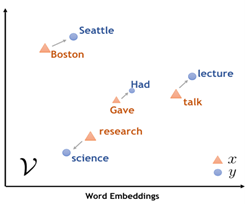
\includegraphics[width=200pt]{images/embed.png}}
\caption{Word Embedding Example\cite{b29}}
\label{Embed}
\end{figure}

\begin{figure}[htbp]
\centerline{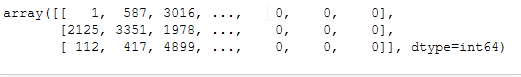
\includegraphics[width=200pt]{images/embed_output.png}}
\caption{Sample Output of Adapted Embedded Model}
\label{EmbedOutput}
\end{figure}

\subsection{Neural Network}
Neural network is widely used in machine learning to develop the correlation between the inputs and outputs. To improve Turkish text classification \cite{b30}, for text summarization and ensemble learning \cite{b31}, to develop short text classification \cite{b32}, for Hierarchical Multi-label Text Classification \cite{b33}, to detect anomaly in the text \cite{b34}, to categorize Bengali text documents \cite{b35}, sentiment categorization 0f social network texts \cite{b36} neural network was employed. A sequential keras model was designed containing encoder (to convert the text into vectors), embedding (to develop relation between words in different context), LSTM (to memorize important information from the words) and neural network (to learn the underlying relationships).

\section{Results and Discussion}
When trying to execute on our planning, we stumbled into a couple of big issues. First, how absolutely massive of an undertaking it was for a 12-week school project. The amount of data cleansing required beyond what was written earlier in this paper is amazingly big for the goal.
\par
There are certain factors that involve the data that change and morph based on time and the scope of what kind of readability score you desire. We predicted some of these problems when coming up the idea for the project and thought that our solutions were simple to implement. We later found out that we could not exactly just implement some parameter filters and call it a day.
\par
The year a paper is written is a huge factor in how readability is calculated. The older the publication, the more different the wording conventions are. A paper written in the 1980s is already vastly different from a paper written in the 90s. Not only from the emerging technology vocabulary but in simple grammar we shifted a lot. We tried to get over this hurdle by filtering our data to only recent papers, but the rapidly changing grammatical climate makes it hard to even pair adjacent years. As you can see at the beginning of Section \ref{datashake}, we also attempted to eliminate special vocabulary that would trip the network’s accuracy too much. This proved to be a fruitless effort because the accuracy still suffered from the many different factors involving this everchanging factor.
\par
The next factor was big and addressed all the way back to our proposal. In the title of the paper, we limited our scoring to only publications made in the Computer Science field. We did this because of the obvious differences in writing between fields. What we did not anticipate was that even within the field, the differences in writing between sub fields were too much for the network to handle and its accuracy suffered when arriving to training in certain subjects.
\par
The obvious solution to all of this is to lower the data amount and narrow the scope of the data. Select a tiny subsection of a field of study with only paper written within the last 5 or so years. Sure, that works, except when it doesn’t. When working with words in a neural network in an attempt to get a good accuracy you need a massive amount of data. We attempted to narrow our scope and use only a small fraction of our original data. The neural network would not pick up from zero accuracy. \\ \\

\section{Conclusion}
As closure, we did a lot of work to preprocess and try to get the project working to an acceptable state. We ultimately could not in our allotted time to work on it. As a team, we plan to try and continue our work done here and potentially get a working scoring network. The project wasn’t impossible and with more time and specific data it is believed that a good result can be achieved. The advancements made here and in future projects on the subjects can produce an interesting and helpful product.

\begin{thebibliography}{00}
\bibitem{b1} Dale, E., \& Chall, J. S. (1949). The concept of readability. Elementary English, 26, 23.
\bibitem{b2} Collins-Thompson, K.: Computational assessment of text readability: A survey of current and future research (2014)
\bibitem{b3} Chall, J.S.: Readability: An appraisal of research and application (34) (1958)
\bibitem{b4} Kincaid, J.P., Fishburne Jr, R.P., Rogers, R.L., Chissom, B.S.: Derivation of new readability formulas for navy enlisted personnel (1975)
\bibitem{b5} Chall, J.S., Dale, E.: Readability revisited: The new Dale-Chall readability formula. Brookline Books (1995)
\bibitem{b6} McNamara, D.S., Graesser, A.C., McCarthy, P.M., Cai, Z.: Automated evaluation of text and discourse with Coh-Metrix. Cambridge University Press (2014)
\bibitem{b7} Schwarm, S.E., Ostendorf, M.: Reading level assessment using support vector machines and statistical language models. In: Proceedings of the 43rd Annual Meeting on Association for Computational Linguistics. pp. 523–530. Association for Computational Linguistics (2005)
\bibitem{b8} Collins-Thompson, K., Callan, J.: Predicting reading difficulty with statistical language models. Journal of the American Society for Information Science and Technology 56(13), 14481462 (2005)
\bibitem{b9} Pitler, E., Nenkova, A.: Revisiting readability: A unified framework for predicting text quality. In: Proceedings of the conference on empirical methods in natural language processing. pp. 186–195. Association for Computational Linguistics (2008)
\bibitem{b10} Pil´an, I., Volodina, E., Zesch, T.: Predicting proficiency levels in learner writings by transferring a linguistic complexity model from expert-written coursebooks. In: Proceedings of COLING 2016, the 26th International Conference on Computational Linguistics: Technical Papers. pp. 2101–2111 (2016)
\bibitem{b11} Xia, M., Kochmar, E., Briscoe, T.: Text readability assessment for second language learners. In: Proceedings of the 11th Workshop on Innovative Use of NLP for Building Educational Applications. pp. 12–22 (2016)
\bibitem{b12} P. Plavén-Sigray, G. J. Matheson, B. C. Schiffler, and W. H. Thompson, “The readability of scientific texts is decreasing over time,” eLife, vol. 6, Sep. 2017. doi: 10.7554/elife 27725. [Online]. Available: http://dx.doi.org/10.7554/eLife.27725.
\bibitem{b13} Hansberry, D.R., Agarwal, N., Shah, R., Schmitt, P.J., Baredes, S., Setzen, M., Carmel, P.W., Prestigiacomo, C.J., Liu, J.K. and Eloy, J.A. (2014), Analysis of the readability of patient education materials from surgical subspecialties. The Laryngoscope, 124: 405-412. https://doi.org/10.1002/lary.24261
\bibitem{b14} Friedman, Daniela B., and Laurie Hoffman-Goetz. “A Systematic Review of Readability and Comprehension Instruments Used for Print and Web-Based Cancer Information.” Health Education \& Behavior 33, no. 3 (June 2006): 352–73. https://doi.org/10.1177/1090198105277329.
\bibitem{b15} Onchonga, David, Sahar Hammoud, Stephen Kuriakose, and Emad Ahmad Khan Muhammad. “Exploring Fear of Childbirth in Kenya through Evaluation of the Readability of Wijma Delivery Expectancy/Experience Questionnaire Version A (W-DEQ-A).” Sexual \& Reproductive Healthcare. Elsevier BV, June 2021. https://doi.org/10.1016/j.srhc.2021.100605.
\bibitem{b16} The New Dale-Chall Readability Formula, https://readabilityformulas.com/new-dale-chall-readability-formula.php.
\bibitem{b17} D. Suleiman and A. Awajan, “Multilayer encoder and single-layer decoder for abstractive Arabic text summarization,” Knowledge-Based Syst., p. 107791, 2021, doi: https://doi.org/10.1016/j.knosys.2021.107791.
\bibitem{b18} T. A. Hilal and H. A. Hilal, “Turkish Text Compression via Characters Encoding,” Procedia Comput. Sci., vol. 175, pp. 286–291, 2020, doi: https://doi.org/10.1016/j.procs.2020.07.042.
\bibitem{b19} N. T. Ly, C. T. Nguyen, and M. Nakagawa, “An attention-based row-column encoder-decoder model for text recognition in Japanese historical documents,” Pattern Recognit. Lett., vol. 136, pp. 134–141, 2020, doi: https://doi.org/10.1016/j.patrec.2020.05.026.
\bibitem{b20} S. T. Klein and D. Shapira, “Pattern matching in Huffman encoded texts,” Inf. Process. Manag., vol. 41, no. 4, pp. 829–841, 2005, doi: https://doi.org/10.1016/j.ipm.2003.08.008.
\bibitem{b21} “Embeddings,” 2021. https://developers.google.com/machine-learning/crash-course/embeddings/video-lecture.
\bibitem{b22} A. Goyal, V. Gupta, and M. Kumar, “A deep learning-based bilingual Hindi and Punjabi named entity recognition system using enhanced word embeddings,” Knowledge-Based Syst., vol. 234, p. 107601, 2021, doi: https://doi.org/10.1016/j.knosys.2021.107601.
\bibitem{b23} S. H. Kumhar, M. M. Kirmani, J. Sheetlani, and M. Hassan, “Word Embedding Generation for Urdu Language using Word2vec model,” Mater. Today Proc., 2021, doi: https://doi.org/10.1016/j.matpr.2020.11.766.
\bibitem{b24} N. Kanakaris, N. Giarelis, I. Siachos, and N. Karacapilidis, “Making personnel selection smarter through word embeddings: A graph-based approach,” Mach. Learn. with Appl., vol. 7, p. 100214, 2022, doi: https://doi.org/10.1016/j.mlwa.2021.100214.
\bibitem{b25} J. Noh and R. Kavuluru, “Improved biomedical word embeddings in the transformer era,” J. Biomed. Inform., vol. 120, p. 103867, 2021, doi: https://doi.org/10.1016/j.jbi.2021.103867.
\bibitem{b26} D. Zhao, J. Wang, Y. Chu, Y. Zhang, Z. Yang, and H. Lin, “Improving biomedical word representation with locally linear embedding,” Neurocomputing, vol. 447, pp. 172–182, 2021, doi: https://doi.org/10.1016/j.neucom.2021.02.071.
\bibitem{b27} S. Li, R. Pan, H. Luo, X. Liu, and G. Zhao, “Adaptive cross-contextual word embedding for word polysemy with unsupervised topic modeling,” Knowledge-Based Syst., vol. 218, p. 106827, 2021, doi: https://doi.org/10.1016/j.knosys.2021.106827.
\bibitem{b28} F. Gasparetti, “Discovering prerequisite relations from educational documents through word embeddings,” Futur. Gener. Comput. Syst., vol. 127, pp. 31–41, 2022, doi: https://doi.org/10.1016/j.future.2021.08.021.
\bibitem{b29} IBM, “Word Mover’s Embedding: Universal Text Embedding from Word2Vec,” 2021. https://www.ibm.com/blogs/research/2018/11/word-movers-embedding/.
\bibitem{b30} M. Aydoğan and A. Karci, “Improving the accuracy using pre-trained word embeddings on deep neural networks for Turkish text classification,” Phys. A Stat. Mech. its Appl., vol. 541, p. 123288, 2020, doi: https://doi.org/10.1016/j.physa.2019.123288.
\bibitem{b31} N. Alami, M. Meknassi, and N. En-nahnahi, “Enhancing unsupervised neural networks based text summarization with word embedding and ensemble learning,” Expert Syst. Appl., vol. 123, pp. 195–211, 2019, doi: https://doi.org/10.1016/j.eswa.2019.01.037.
\bibitem{b32} P. Wang, B. Xu, J. Xu, G. Tian, C.-L. Liu, and H. Hao, “Semantic expansion using word embedding clustering and convolutional neural network for improving short text classification,” Neurocomputing, vol. 174, pp. 806–814, 2016, doi: https://doi.org/10.1016/j.neucom.2015.09.096.
\bibitem{b33} X. Zhang, J. Xu, C. Soh, and L. Chen, “LA-HCN: Label-based Attention for Hierarchical Multi-label Text Classification Neural Network,” Expert Syst. Appl., vol. 187, p. 115922, 2022, doi: https://doi.org/10.1016/j.eswa.2021.115922.
\bibitem{b34} J. Mu, X. Zhang, Y. Li, and J. Guo, “Deep neural network for text anomaly detection in SIoT,” Comput. Commun., vol. 178, pp. 286–296, 2021, doi: https://doi.org/10.1016/j.comcom.2021.08.016.
\bibitem{b35} M. R. Hossain, M. M. Hoque, N. Siddique, and I. H. Sarker, “Bengali text document categorization based on very deep convolution neural network,” Expert Syst. Appl., vol. 184, p. 115394, 2021, doi: https://doi.org/10.1016/j.eswa.2021.115394.
\bibitem{b36} X. Liu, T. Tang, and N. Ding, “Social network sentiment classification method combined Chinese text syntax with graph convolutional neural network,” Egypt. Informatics J., 2021, doi: https://doi.org/10.1016/j.eij.2021.04.003.
\end{thebibliography}

\end{document}
